\setlength{\abovedisplayshortskip}{0pt}
\chapter{Theory}
\label{chap:theory}

\section{The Standard Model}
The SM is currently considered the best available theoretical description of the
fundamental particles as well as three of the four known fundamental forces of
the universe, with gravity being the only exception. In the quantum mechanical
description of the universe, classical point particles are replaced by
wavefunctions that evolve according to the Schr\"odinger equation and describe
the probability of a measurement outcome. In contrast, the SM is a Quantum Field
Theory (QFT), which applies quantum mechanics to classical \textit{fields}.
These fields are continuous mathematical objects that specify a value or vector
at each spacetime point. Quantum fields may have localized excitations, or
ripples, that can be thought of as \textit{particles}. The SM includes a set of
fields whose excitations, or particles, are fundamental in that they are not
expected to be approximations of alternative field descriptions at smaller
distance scales. The SM is relativistic in the sense that its equations of
motion are Lorentz invariant. In other words, they do not depend on the choice
of inertial frame. If that were not the case, the laws of physics could depend
on an arbitrary choice of reference frame.

Fundamental particles in the SM can be classified by how their joint
wavefunctions behave under interchange of two identical particles:
\textit{bosons}, whose wavefunctions do not change under such exchange have
integer values of the quantum number corresponding to intrinsic angular momentum
(i.e., \textit{spin}\footnote{Spin is a multiple of the reduced Planck constant
$\hbar$, but throughout this work natural units will be used for which $c =
\hbar = 1$.}), while \textit{fermions}, whose wavefunctions change sign under
exchange of two identical particles have half-integer spin. A profound
implication of this difference is that no two fermions can occupy the same
quantum state, while no such restriction exists for bosons. Fundamental
particles can have one of two possible chiralities. This intrinsic property
specifies the direction in which the quantum phase rotates in the complex plane
(clockwise is referred to as left-handed, and counterclockwise as right-handed).
Fundamental particles are further characterized by their mass and by quantum
numbers called \textit{charges} that determine which of the fundamental forces
they participate in.

Fermions are divided into two groups: quarks and leptons. Quarks carry
\textit{color} charge, indicating that they participate in the strong
interaction, while \textit{leptons} do not. Quarks also carry an electric charge
and therefore participate in the electromagnetic interaction. They can be of an
\emph{up-type}, with an electric charge of $+\frac{2}{3}\abs{\Pe}$, or a
\emph{down-type}, with an electric charge of $-\frac{1}{3}\abs{\Pe}$. Leptons
likewise can be \emph{electron-type} or \emph{neutrino-type}. Electrons carry an
electric charge of $-\abs{\Pe}$ while neutrinos have no electric charge.

There are three \textit{generations}\footnote{Note that the number of
generations is an experimentally driven feature of the SM; there is no
theoretical justification for why there should be exactly three generations.} of
fermions, which are identical except for mass. Each generation consists of an
up-type quark, a down-type quark, an electron-type lepton, and a neutrino-type
lepton. The more massive generations are not stable, and ordinary matter is
consequently made up of first-generation particles. For each fermion, a
corresponding antifermion with the same mass but with opposite charge exists.
Charged massive fermions are described by Dirac spinors, which have a component
for each of the two chirality states. The uncharged fermions, the neutrinos,
carry only left-handed chirality (anti-neutrinos carry right-handed chirality).
Properties of the fundamental fermions are summarized in~\cref{tab:fermions}.

Because spin is conserved, a fermion with a spin projection of $+\frac{1}{2}$
may emit a boson with a spin of 1 and remain a fermion with a spin projection of
$-\frac{1}{2}$.  Similarly, a boson with integer spin can emit a boson and will
remain a boson. However a fermion cannot emit another fermion because this would
leave a particle with integer spin. Consequently, only bosons can be
``exchanged", that is, emitted or absorbed while leaving the emitter or absorber
intact.

The fundamental forces result from couplings between fundamental fields. For
example, the force between two excitations of a fermionic field is mediated by
an excitation of a fundamental bosonic field to which it is coupled, which can
be understood as an interaction in which a boson is exchanged between two
fermions. It should be noted that a force is understood to be involved more
generally in any interaction involving the excitation of a bosonic field. For
example, radioactive beta decay is a weak force process because it necessarily
involves the emission of a bosonic excitation of one of the fields associated
with the weak force.

All massive particles interact gravitationally; however, gravity is such a weak
force that it is irrelevant and undetectable in particle interactions at the
LHC. The gravitational interaction is not described in the SM. The
electromagnetic interaction, responsible for binding electrons in atoms, is
mediated through the exchange of an excitation of the electromagnetic field, a
\textit{photon} ($\gamma$), which is electrically neutral and massless. Because
the photon is massless, the range of the electromagnetic force is infinite. The
strong force is responsible for holding quarks together to form \textit{hadrons}
and for binding protons and neutrons together to form atomic nuclei. It is
mediated via the exchange of massless bosons called gluons. The weak force,
responsible for the decay of heavier fermion generations into lighter ones, is
mediated by the $\text{W}^+$, $\text{W}^-$, and Z bosons. The W and Z bosons,
discovered at CERN in 1983~\cite{ARNISON1983103,BANNER1983476}, play a special
role in this thesis. The Higgs field is a scalar field with a non-zero
expectation value that permeates all space. Excitations of this field (the Higgs
boson) couple to the W and Z bosons and the fermions to give them mass.

\begin{table}[tb]
  \begin{threeparttable}
  \caption[Fermions of The Standard Model]{
    Fermions of the Standard Model
  }
  \label{tab:fermions}
  \sisetup{quotient-mode=fraction}
  \begin{tabular}{
      llc
      S[table-format=<3.3e+1]
    cc}
    \toprule
    &          & Symbol                    & {Mass / \si{\GeV}} & {Electric charge / $\abs{\Pe}$} & {\(T_3\)} \\
    \midrule
    \multirow{6}{*}{\tikz \node[rotate=90] {Quarks};}
    & up       & \Pu                       & 2.2e-3             & \(+\,\frac23\)         & \(+\,\frac12\) \\
    & down     & \Pd                       & 4.7e-3             & \(-\,\frac13\)         & \(-\,\frac12\) \\
    & charm    & \Pc                       & 1.28               & \(+\,\frac23\)         & \(+\,\frac12\) \\
    & strange  & \Ps                       & 0.096              & \(-\,\frac13\)         & \(-\,\frac12\) \\
    & top      & \Ptop                     & 173.1              & \(+\,\frac23\)         & \(+\,\frac12\) \\
    & bottom   & \Pb                       & 4.18               & \(-\,\frac13\)         & \(-\,\frac12\) \\
    \midrule
    \multirow{4}{*}{\tikz \node[rotate=90] {Leptons};}
    & electron & \Pe                       & 0.51e-3            & \(-\,1\)               & \(-\,\frac12\) \\
    & muon     & \Pmu                      & 0.106              & \(-\,1\)               & \(-\,\frac12\) \\
    & tau      & \Ptau                     & 1.777              & \(-\,1\)               & \(-\,\frac12\) \\
    & neutrino & \(\Pnu_{\Pe,\Pmu,\Ptau}\) & < 20e-3            & \(\phantom{+}\,0\)     & \(+\frac12\) \\
    \bottomrule
  \end{tabular}
\end{threeparttable}

\end{table}

\subsection{The Lagrangian formulation and principle of stationary action}
The \textit{Lagrangian density} $\mathcal{L}$ (hereafter, simply the Lagrangian)
is a functional that takes the configuration of one or more fields $\phi_i$ and
their derivatives $\partial_\mu\phi_i$ and outputs a number. The Lagrangian
encodes the system's dynamics. A sequence of configurations in spacetime
comprise a \textit{path}. The integral of the Lagrangian along a given path in
spacetime is called that path's \textit{action}\footnote{See
~\cite{Klauber:1550150} chapter 18 for a good introductory discussion of this
topic.} and is proportional to the change in complex phase accrued along that
path:
\begin{equation}
S = \int \mathcal{L} d^4x
\end{equation}
where $x^\mu = (t, x, y, z)$. One of Feynman's remarkable insights was that a
system evolving from an initial to a final configuration can be considered as
following all possible paths between them (even those paths that do not satisfy
usual physical laws) and that each possible path is equally probable. When the
paths are added together, those in which the action is \textit{stationary}
(i.e., in which considering small variations to arbitrary neighboring paths
produces no change in the action) tend to add constructively, while the variance
in the other paths' actions are large and random such that those paths add
incoherently. As a result, the most highly weighted path is the one in which the
action is stationary. This is called the \textit{principle of stationary
action}, although in most cases the path of stationary action minimizes the
action. A prominent historical example is the observation by Fermat that light
follows the path of least time (in the case of light, time is proportional to
action).

\subsection{Symmetry and gauge invariance}
\label{sec:symmetry}
Symmetry (i.e., invariance under transformation) seems to play a profound role
with respect to the laws of nature. Symmetries can be either continuous or
discrete. Rotation of a square is an example of a discrete transformation: only
90, 180, and 270 degree turns are symmetric. Rotation of a circle is an example
of a continuous symmetry: after a rotation of any arbitrary angle, the circle
looks the same as before. Continuous transformations can be represented by
\textit{Lie groups}, in which an infinitesimal transformation $g$, expressed in
terms of infinitesimal parameters $\alpha^a$, is an infinitesimal perturbation
of the identity transformation: $g(\alpha) = \mathbf{1} + i\alpha^aT^a +
\mathcal{O}(\alpha^2)$, where the Hermitian operators $T^a$ are the
\textit{generators} of the group. Finite transformations can be constructed from
the repeated application of such infinitesimal transformations.

A Lagrangian exhibits a continuous symmetry if it is invariant under a
transformation of fields $\phi_i(x) \rightarrow \phi_i^\prime(x) = U_{ij}
\phi_j(x)$. If the continuous transformation $U_{ij}$ is constant at every point
$x$ in spacetime it is said to be \textit{global}. Noether's first theorem
states that a global continuous symmetry in the Lagrangian implies that an
associated quantity is conserved. For example, invariance with respect to
translations in time gives rise to the conservation of energy, invariance with
respect to translations in space gives rise to the conservation of momentum, and
invariance with respect to rotations in space gives rise to conservation of
angular momentum. In electrodynamics, the Lagrangian is invariant under global
phase transformations, which gives rise to the conserved electric charge.

Ordinary transformations connect physically inequivalent states, leaving
observables unchanged. If a ball is thrown inside a train car, the calculation
of its trajectory will be invariant with respect to the train car's velocity,
even though different velocities correspond to different physical states. In
contrast, a \textit{gauge} transformation only changes our mathematical
description and does not connect different physical states. Field theories
describe fields that are not directly measured; instead, measurements are made
of various observables such as energies, velocities, and charges. Different
configurations of the underlying fields (i.e., different \textit{gauges}) may
possibly lead to the same set of observations; there is an inherent redundancy.
If the observable quantities of a physical theory do not change when a gauge
transformation is performed (i.e., one possible gauge configuration is
transformed to another), then the physical theory is said to be gauge invariant.

The SM is based on the requirement that the theory be invariant under certain
types of \textit{local} continuous gauge transformations $U_{ij}(x)$, which
unlike the global transformation $U_{ij}$, can vary from point to point. The
program of insisting that the theory respect some set of local gauge symmetries
is called \textit{gauge theory}, and the procedure used to enforce the symmetry
on the fermionic fields necessitates the existence of additional \textit{gauge
fields}, bosonic fields that are associated with the SM forces.

To see how this works, consider the Dirac Lagrangian for a fermion:
\begin{equation}
  \mathcal{L} = \bar{\psi}(i\gamma^\mu \partial_\mu - m) \psi
  \label{eq:dirac}
\end{equation}
where $m$ is the mass associated with a spin-1/2 particle $\psi$, $\gamma^\mu$ are the Dirac matrices, and $\bar{\psi}$ is the Hermitian conjugate of $\psi$.  This Lagrangian is invariant under the global transformation of the $U(1)$ group $\psi \rightarrow e^{iq\theta} \psi$, where $q$ is the charge of the particle involved, which is conserved via Noether's theorem. If we consider a local transformation $\psi \rightarrow e^{iq\theta(x)} \psi$ which varies from point to point, we see that the Lagrangian is no longer invariant because of the derivative in first term:
\begin{align}
  \partial_\mu(e^{iq\theta}\psi)
  &= iq\partial_\mu \theta e^{iq\theta}\psi + e^{iq\theta}\partial_\mu\psi.
\end{align}
For the Lagrangian this means that
\begin{align}
  \mathcal{L} &\rightarrow
    - q \bar{\psi}\gamma^\mu \partial_\mu \theta \psi
    + \bar{\psi}i\gamma^\mu \partial_\mu\psi
    - m \bar{\psi} \psi \\
  &\rightarrow
  \mathcal{L}
    - q \bar{\psi} \gamma^\mu \partial_\mu \theta \psi.
  \label{eq:unsymmetric}
\end{align}
Clearly the invariance has been spoiled, but a general procedure is known to
recover the symmetry. The derivative in~\cref{eq:dirac} is replaced with the
\textit{covariant derivative},
\begin{align}
  D_\mu &= \partial_\mu - i q A_\mu,
\end{align}
which includes an additional term whose role is to produce a cancellation of the
term in~\cref{eq:unsymmetric} that spoiled the invariance. This procedure has
resulted in the addition of a new vector field $A_\mu$, transforming as $A_\mu
\rightarrow A_\mu-\partial_\mu \theta$, which has been coupled to the fermionic
field through cross terms in~\cref{eq:dirac}. Because a new field has been added
to the theory, a corresponding kinetic term must be added to describe the
propagation of a vector field of mass $m$ to the Lagrangian:
\begin{align}
  \mathcal{L_\text{free}} =
    - \frac{1}{4}(\partial^\mu A^\nu
    - \partial^\nu A^\mu)(\partial_\mu A_\nu - \partial_\nu A_\mu)
    + m^2A^\mu A_\mu.
\label{eq:proca}
\end{align}
The factors in the first term transform as
\begin{align}
  \partial^\mu A^\nu - \partial^\nu A^\mu
  &\rightarrow \partial^\mu (A^\nu - \partial^\nu \theta)
  - \partial^\nu (A^\mu - \partial^\mu \theta) \\
  &\rightarrow \partial^\mu A^\nu - \partial^\mu A^\mu
\end{align}
and so are invariant under the gauge transformation. The second term transforms
as $m^2A^\mu A_\mu \rightarrow m^2A^\mu A_\mu - 2 m^2 A^\mu \partial_\mu
\theta$. Therefore, to leave the Lagrangian invariant for arbitrary $\theta$, we
must have $m=0$. Thus, starting from the globally invariant Dirac Lagrangian for
fermions and requiring that it be locally invariant\footnote{Indeed, it seems
unnatural \textit{not} to require local invariance, as spacelike-separated
points cannot communicate with each other; the alternative suggests action at a
distance.}, a new massless vector field has arisen as a matter of necessity.
Putting everything together and identifying the electromagnetic field tensor
$F^{\mu\nu} = \partial^\mu A^\nu-\partial^\nu A^\mu$ we recognize this result as
the quantum electrodynamics (QED) Lagrangian:
\begin{align}
  \mathcal{L}_{QED}
    &= \bar{\psi}(i\gamma^\nu D_\mu - m)\psi
      - \frac{1}{4}F_{\mu\nu} F^{\mu\nu} \\
    &= \bar{\psi}(i\gamma^\nu \partial_\mu - m)\psi
      - \frac{1}{4}F_{\mu\nu}F^{\mu\nu}
      + q\bar{\psi}\gamma^\mu\psi A_\mu
\end{align}
where $q$ is the electric charge, and the final term describes the interaction
between the photon field and charged fermions. QED is an example of an
\textit{abelian} gauge theory because successive applications of the generator
(i.e., successive changes in the phase) commute with one another: the order in
which they are applied can be reversed without changing the result.

\subsection{The Standard Model Lagrangian}
QED has been remarkably successful, but to make further progress we must also
consider non-abelian gauge theories for which the generators $T^a$ do not
commute:
\begin{equation}
  [T^a, T^b] = if^{abc} T^c,
  \label{eq:generatorcommutation}
\end{equation}
where $f^{abc}$ are called the structure constants. In the following sections
the electroweak and quantum chromodynamics (QCD) sectors are discussed
separately, but it is helpful to first note the common elements that are
required. In each case we need to determine 1) which gauge group specifies the
vector fields, 2) which fields are present, 3) how the fields transform under
the group, and 4) a locally gauge-invariant Lagrangian in terms of the fields.
For each group, a representation $t^a$ is first chosen for the generators of the
group. Next, we demand that the theory be invariant under a local $SU(N)$
transformation\footnote{A unitary group $U(N)$ is a group of $N \times N$
unitary matrices, where a unitary matrix is one for which the conjugate
transpose equals the matrix inverse; these groups have a special importance in
physics because they preserve norms.  A special unitary group has the additional
property that the determinant of each group element is 1. A unitary group has
$N^2$ generators. For a special unitary group, the condition of unitarity
reduces the number of independent elements by one, so a special unitary group
has $N^2-1$ generators.}, $\psi \rightarrow \psi^\prime = e^{i\alpha^a(x)t^a}
\psi$, where $\alpha^a(x)$ are arbitrary functions of $x$.

Similarly, as was introduced in~\cref{sec:symmetry}, the covariant derivative
$D_\mu = \partial_\mu-igA^a_\mu t^a$ introduces a new coupling constant $g$
parameterizing the strength of the interaction and vector field $A_\mu^a$ for
each generator of the local symmetry. The field tensor is defined in terms of
the covariant derivative:
\begin{align}
  - igF^a_{\mu\nu}t^a
    &= \comm{D_\mu}{D_\nu} \label{eq:fieldtensorcommutator} \\
    &= \comm{\partial_\mu - igA^a_\mu t^a}{\partial_\nu-igA^b_\nu t^b} \\
    &= \comm{\partial_\mu}{\partial_\nu}
      - ig\comm{A_\mu^a t^a}{\partial_\nu}
      - ig\comm{\partial_\mu}{A_\nu^b t^b}
      + (ig)^2\comm{A_\mu^b t^b}{A_\nu^c t^c} \\
    &= ig\left[\partial_\nu A_\mu^a
      - \partial_\mu A_\nu^a
      + (ig)if^{abc}A_\mu^b A_\nu^c \right] t^a \\
    \rightarrow F^a_{\mu\nu}
    &= \partial_\mu A_\nu^a
      - \partial_\nu A_\mu^a
      + gf^{abc}A_\mu^b A_\nu^c.
  \label{eq:fieldtensor}
\end{align}

Note that the final term in the field tensor appears as a result of the
non-commutative nature of the generators of $SU(N)$. It indicates that when the
kinetic term is expressed as in~\cref{eq:proca}, terms arise with three and four
factors of the vector field. These factors are the gauge boson self-interactions
which do not appear in abelian theories such as QED. Note also that a gauge
field has emerged corresponding to each generator of the group. The symmetry
group used in the case of QED is $U(1)$, which has a single generator and a
single gauge field. In addition, Noether's theorem results in a single conserved
charge. $SU(N)$ has $N^2-1$ generators; therefore, an $SU(N)$ gauge theory has
$N^2-1$ gauge fields, and application of Noether's theorem yields $N$ conserved
charges.

The SM is based on the product of two special unitary groups and one unitary
group: $SU(3) \times SU(2) \times U(1)$. The $SU(3)$ group describes the strong
interactions, while the $SU(2) \cross U(1)$ group describes both the weak and
electromagnetic interactions.

\subsection{Quantum chromodynamics}
QCD, which provides a successful description of the strong interaction, emerges
when the Lagrangian is required be invariant under local transformations of the
non-abelian gauge group $SU(3)_C$.

Because it is $SU(N)$ with $N=3$, there are three conserved charges, referred to
as \textit{color} charges \textit{red}, \textit{green}, and \textit{blue}.
Similarly, there are $N^2-1=8$ generators of the group corresponding to the
eight gauge fields, called \textit{gluons}. Leptons, which carry no color
charge, do not interact via the strong force. Each quark flavor can be expressed
as a color triplet:
\begin{equation}
  q = \left(
    \begin{array}{c}
      q_r \\
      q_g \\
      q_b
    \end{array}
  \right),
\end{equation}
where the $q_x$ are Dirac spinors and the subscripts label the color states. The QCD Lagrangian is
\begin{align}
  \mathcal{L}_{QCD} &= \mathcal{L}_{gluon} + \mathcal{L}_{quark}\text{, with} \\
  \mathcal{L}_{gluon} &= - \frac{1}{4}\sum_{a=1}^8 G^a_{\mu\nu} G_a^{\mu\nu},
\end{align}
where the field strength tensor is defined similarly
to~\cref{eq:fieldtensorcommutator}:
\begin{align}
  -ig_sG^a_{\mu\nu}t^a
    &= \comm{D_\mu}{D_\nu}\text{, with} \\
  D_\mu^{ij}
    &= \partial_\mu\delta_{ij} - i g_s t^a_{ij}G^\mu_a \\
  \rightarrow G^a_{\mu\nu}
  &= \partial_\mu G^a_\nu
    - \partial_\nu G^a_\mu
    - g_s f^{abc} G^b_\mu G^c_\nu,
  \label{eq:gluonfieldtensor}
\end{align}
where $t^a$ are the generators of $SU(3)$, the $i$s and $j$s are color indices
running from 1 to 3, the sum over $a$ runs from 1 to 8, $G^a_\mu$ are the gluon
fields, $g_s$ is the strong coupling constant, and $f^{abc}$ are the structure
constants of SU(3) defined by the commutation relation between the generators of
SU(3). As carriers of color charge, gluons can couple to one another; this
``self-interaction" arises from the last term in~\cref{eq:gluonfieldtensor}.

The quark Lagrangian is
\begin{equation}
  \mathcal{L}_{quark}
    = \sum_{f} \bar{q}_i^{(f)}
      \left(
        i\gamma_\mu D^\mu_{ij} - m_f\delta_{ij}
      \right)q_{j}^{(f)}
\end{equation}
where the sum over $f$ corresponds to the six quark flavors and $i$ and $j$ again refer to the three colors.

\subsubsection{Confinement and hadronization}
\label{sssec:hadronization}
Unlike in QED, the force between quarks is large at large separations and does
not become weaker with increasing separation. Conversely, quarks separated by
short distances (e.g., during high energy scattering) are only weakly coupled.
This striking feature of QCD is called \emph{asymptotic freedom}. To understand
this concept, it is helpful to draw an analogy to QED. When a photon propagates
through the vacuum, it can induce the production of virtual pairs of electrons
and positrons (called vacuum fluctuations) that have a \emph{screening} effect,
making the interaction coupling weaker at larger distances (similar to how the
force between two electrons is effectively reduced when submerged in a
dielectric medium). QCD has the same screening effect due to the production of
quark-antiquark pairs, which tends to make the interaction coupling decrease
with increasing distance. Unlike the electrically neutral photons in QED,
however, gluons carry color charge. This charge leads to additional
\emph{anti-screening} effects from nonlinear self-interactions between the
gluons, making the interaction coupling larger at large distances. In his Nobel
prize lecture~\cite{RevModPhys.77.857}, Wilczek uses the analogy of a
thundercloud, where a small charge induces a cloud of virtual particles in a
self-reinforcing process. The cloud gets bigger as one moves away from the
source, enhancing its power. This \emph{running coupling constant} means that
QCD can only be calculated perturbatively at large momentum transfers with $q^2
\gg \Lambda_\text{QCD}$, where $\Lambda_\text{QCD} \sim \SI{250}{MeV}$.

A consequence of asymptotic freedom at low energies is \textit{color
confinement}: quarks and gluons do not exist in isolation at distances larger
than $1/\Lambda_\text{QCD}$. As an example, consider trying to pull apart a
stable, color-neutral meson (quark-antiquark pair). As the two quarks are
separated, the energy in the gluon field between them grows until it is
energetically favorable to produce a quark-antiquark pair that combines with the
original quark and antiquark to form two separate mesons. The collision energies
at the LHC are high enough (corresponding to short interaction distances) that
the collisions are between quarks and gluons rather than protons. After
high-energy quarks or gluons emerge from such a collision, they undergo two
separate processes. First, a \textit{shower} of quarks is produced due to the
tendency of quarks to radiate gluons and gluons to in turn produce
quark-antiquark pairs. Second, due to the process of color confinement, the
shower of isolated quarks recombine or combine with quark-antiquark pairs,
produced from the energy in the above-mentioned gluon field between separated
quarks, to ultimately result in a collimated ``spray" of hadrons called a
\textit{jet}. The total energy of the jet reflects the energy of the quark or
gluon that initiated it. Because jets are showers of hadrons that do not
unambiguously reflect the nature of the quark or gluon that initiated them, and
because jets are produced so commonly in high energy proton collisions, they
result in challenging backgrounds for many LHC analyses.

\subsection{Electroweak interactions}
\label{sec:electroweak}
A unified description of the weak and electromagnetic forces was proposed by
Glashow~\cite{GLASHOW1961579}, Salem~\cite{Salam:1968rm}, and
Weinberg~\cite{PhysRevLett.19.1264}, and it results from the assumption of
invariance under an $SU(2) \cross U(1)$ gauge symmetry.  The $SU(2)$ symmetry
gives rise to the conserved weak isospin charge with three corresponding
massless bosons ($W_1$, $W_2$, and $W_3$), and the $U(1)$ symmetry gives rise to
the conserved weak hypercharge and its associated massless $B$ boson.
\Cref{ssec:SSB} covers how these bosons relate to the familiar bosons of the
electromagnetic and weak interactions.

A major difference between the weak force and the other fundamental forces is
that the weak force is a \textit{chiral} theory: it does not conserve
\textit{parity} (i.e., inversion of spatial coordinates). Consequently, to
specify the field content it is necessary to split it into left- and
right-handed components, which can be accomplished via the \emph{projection
operators}:
\begin{align}
  \psi_L &= \frac{1}{2}(1-\gamma^5)\psi \\
  \psi_R &= \frac{1}{2}(1+\gamma^5)\psi,
\end{align}
where the right-handed fermions do not participate in the weak interaction. For
this reason, the weak isospin group is referred to as $SU(2)_\text{L}$.
Mathematically, this is encoded in the transformation properties of the two
types of fermions: right-handed fermions transform as isospin singlets ($I=0$)
and left-handed fermions transform as isospin doublets ($I=\frac{1}{2}$):
\begin{align}
  Q^i_L &= \left(
    \begin{array}{c}
      u^i_L \\
      d^i_L
    \end{array}
  \right),\,
  E^i_L = \left(
    \begin{array}{c}
      \nu^i_L \\
      l^i_L
    \end{array}
  \right), \\
  f^i_R &= e^i_R, u^i_R, d^i_R
\end{align}
where $i$ runs over the three fermion generations. Note that in this formulation, the fundamental fermions are all massless because a mass term would not be gauge invariant. The mass term is
\begin{align}
  -m_f\bar{\psi}\psi &= -m_f(\bar{\psi}_R + \bar{\psi}_L)(\psi_R + \psi_L) \\
                     &= -m_f(\bar{\psi}_R\psi_L+\bar{\psi}_L\psi_R).
  \label{eq:fermion_mass}
\end{align}
This expression is not gauge invariant because $\psi_L$ changes under isospin rotations while $\psi_R$ does not. The mechanism by which the fermion masses arise is explained in the following section. The covariant derivative $D_\mu$ is
\begin{equation}
  D_\mu = \partial_\mu - i g \frac{1}{2} W_\mu^a\sigma^a - i \frac{1}{2}g^\prime B_\mu
  \label{eq:electroweak_derivative}
\end{equation}
where the $a$ index runs from 1 to 3 over the generators of $SU(2)$ and
\begin{align}
  \sigma^a &= \text{Pauli matrices} \\
  B_\nu &= \text{$U(1)$
  gauge field} \\
  W_\mu^a &= \text{3 $SU(2)$ gauge fields} \\
  g^\prime &= \text{$U(1)$ coupling constant} \\
  g &= \text{$SU(2)$ coupling constant}.
\end{align}

A three-dimensional \emph{weak isospin} space is defined by the three generators
$\sigma^a$; global $SU(2)$ transformations correspond to rotations of the
$W_\mu^a$ vectors in this space. The Lagrangian describing the massless gauge
fields is given by the following:
\begin{equation}
  \mathcal{L}_{gauge} = - \frac{1}{4} W^a_{\mu\nu} W_a^{\mu\nu}
  - \frac{1}{4}B_{\mu\nu}B^{\mu\nu}
\end{equation}
where the field strength tensors $W^a_{\mu\nu}$ and $B^{\mu\nu}$ are defined as
\begin{align}
  B_{\mu\nu} &= \partial_\mu B_\nu - \partial_\mu B_\mu, \\
W^a_{\mu\nu} &= \partial_\mu W_\nu^a - \partial_\nu W_\mu^a + g f^{abc}W^b_\mu W^c_\nu.
\end{align}
To complete the picture, we add a term to describe how matter interacts with the $B_\nu$ and $W_\mu^a$ fields:
\begin{equation}
  \mathcal{L}_{int} = \sum_{i,f}\bar{f^i}(i\gamma^\mu D_\mu)f^i,
\end{equation}
where $i=1,2,3$ refers to the three fermion generations, and $f=E^i_L, Q^i_L, e^i_R, u^i_R, d^i_R$. The electroweak sector is then described by $\mathcal{L}_{EW} = \mathcal{L}_{gauge} + \mathcal{L}_{int}$. This completes the description of an electroweak sector that is flawed in several respects. First, all four gauge bosons are massless, while the observed gauge bosons associated with the weak force are massive. In addition, there are four conserved charges, while the observed electroweak sector conserves only electric charge and the third component of weak isospin. Further, as we saw in~\cref{eq:fermion_mass}, the chiral nature of the weak interaction implies that none of the SM fermions that participate in the weak interaction can have mass. In the next section, these seemingly grave problems are addressed.

\subsection{Spontaneous symmetry breaking}
\label{ssec:SSB}
Within the SM, as long as the $SU(3) \cross SU(2) \cross U(1)$ symmetry is exact, all gauge bosons should be massless as shown in~\cref{sec:symmetry} and the fermions should be massless as shown in~\cref{sec:electroweak}. However, these outcomes are in conflict with the experimental evidence: the $SU(2)$ bosons and the fermions have been observed to have mass.

In order for the fundamental fermions and gauge bosons to acquire mass, the
gauge symmetry must somehow be broken, which occurs through a mechanism called
\textit{spontaneous symmetry breaking} (SSB). SSB is ``spontaneous" in the sense
that no outside cause of the symmetry breaking is present. For a skydiver
falling to the ground, gravity breaks the symmetry, making up and down different
from left and right. In SSB, the state of the system is not symmetric, but the
laws of physics remain so. As a classical example of SSB, consider a ball placed
at the top of the surface in~\cref{fig:mexican_hat} subject to gravitational
force pointing downward along the axis of symmetry. The Lagrangian of the system
is symmetric with respect to rotations around the central axis, but the ball is
unstable due to quantum fluctuations (i.e., Heisenberg's uncertainty relations
require that the wave function of the ball cannot be indefinitely localized). To
reach the stable ground state, the system must spontaneously break the
rotational symmetry, with the ball rolling to the bottom. In the ground state,
the ball and the surface individually still possess rotational symmetry, but the
system as a whole does not. Another example is the orbit of the moon around the
Earth. Newton's laws are rotationally invariant, but the solution of these laws
that describe the moon's motion is not; it depends on initial conditions, so the
rotational symmetry of the underlying law is not manifest.

\begin{figure}[tb]
  % see https://tex.stackexchange.com/questions/229178/how-to-draw-this-particular-mexican-hat-potential
% TODO: make bigger
\pgfdeclarefunctionalshading{sphere}{
  \pgfpoint{-25bp}{-25bp}}{
  \pgfpoint{25bp}{25bp}}{}{
    25 div exch
    25 div exch
    2 copy
    dup mul exch
    dup mul add
    1.0 sub
    0.3 dup mul
    -0.5 dup mul add
    1.0 sub
    mul abs sqrt
    exch 0.3 mul add
    exch -0.5 mul add
    dup abs add 2.0 div
    0.6 mul 0.4 add
    dup
    0.4
}
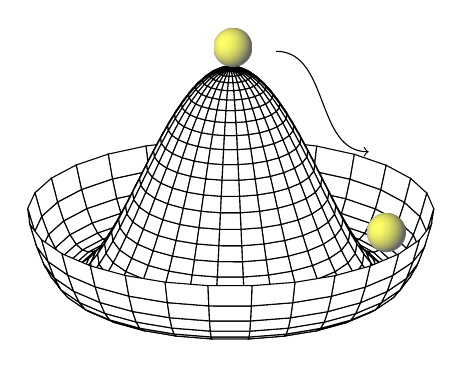
\begin{tikzpicture}
  \begin{axis}[
    hide axis,
    samples=30,
    domain=0:360,
    y domain=0:1.25
    ]
    \addplot3 [surf, shader=flat, draw=black, fill=white, z buffer=sort] ({sin(x)*y}, {cos(x)*y}, {(y^2-1)^2});
  \end{axis}
  \shade[shading=sphere] (3.45, 4.45) circle [radius=0.25cm];
  \shade[shading=sphere] (5.4, 2.1) circle [radius=0.25cm];
  \node[anchor=east] at (4.0, 4.4) (text) {};
  \node[anchor=south] at (5.3, 3.0) (description) {};
  \draw (description) edge[out=180, in=0,<-] (text);
\end{tikzpicture}

  \caption[Spontaneous symmetry breaking (classical example)]{
    A classical example of an SSB is obtained by considering the
    motion of a ball placed at the top of this surface.
  }
  \label{fig:mexican_hat}
\end{figure}

The fact that the fermion and vector bosons have mass indicates that SM gauge
invariance must be spontaneously broken. However, the electric charge is
observed to be conserved and the photon is observed to be massless, so whatever
SSB the SM observes should preserve $SU(3)_\text{c} \times U(1)_\text{EM}$.

To see how this can be accomplished\footnote{This section follows the
derivations
in~\cite{Griffiths:111880,Romanino:2009zz,cottingham1998introduction}.}, it is
important to note that the description of field fluctuations assumes
fluctuations with respect to some ground state, that is, a configuration that
has minimum energy. In the previous discussion the implicit assumption is that
the lowest-energy field configuration is $\phi=0$, so that trivially the vacuum
expectation value is invariant under the symmetry. SSB will arise if $\phi=0$ is
not the ground state.

To see how this works, consider the case of a complex scalar field $\phi =
\phi_1 + i\phi_2$ with the Lagrangian
\begin{align}
  \mathcal{L} &=
    (\partial_\mu\phi)^\dagger (\partial^\mu\phi)
    - U(\phi^\dagger\phi),\
  U(\phi^\dagger\phi) =
    \frac{1}{2}\mu^2\phi^\dagger\phi
    + \frac{1}{4}\lambda(\phi^\dagger\phi)^2.
  \label{eq:complex_lagrangian}
\end{align}
\begin{figure}[tb]
  \begin{subfigure}{0.33\textwidth}
    \centering
    \includegraphics[width=\textwidth]{figures/complex_scalar_neg_lambda}
    \caption{}
    \label{sfig:neg_lambda}
  \end{subfigure}%
  \begin{subfigure}{0.33\textwidth}
    \centering
    \includegraphics[width=\textwidth]{figures/complex_scalar_pos_mass}
    \caption{}
    \label{sfig:pos_mass}
  \end{subfigure}%
  \begin{subfigure}{0.33\textwidth}
    \centering
    \includegraphics[width=\textwidth]{figures/complex_scalar_neg_mass}
    \caption{}
    \label{sfig:neg_mass}
  \end{subfigure}
  \caption[Potential of a complex scalar field]{
    The potential for a complex scalar field given $\lambda < 0$ \subref{sfig:neg_lambda},
     $\mu^2 > 0$~\subref{sfig:pos_mass}, and $\mu^2 < 0$~\subref{sfig:neg_mass}.
  }
  \label{fig:complex_potential}
\end{figure}
This Lagrangian is invariant under the global $U(1)$ phase transformation $\phi
\rightarrow e^{i\theta}\phi$. What are the constraints on $\mu^2$ and $\lambda$?
If $\lambda$ is negative, the potential will not be bounded from below
(see~\cref{fig:complex_potential}~\subref{sfig:neg_lambda}); such a system would
be unstable and have no defined ground state. There is no such constraint on
$\mu^2$; as shown in~\cref{fig:complex_potential}~\subref{sfig:pos_mass}, there
is one minimum in the case that $\mu^2>0$, and there are degenerate minima along
a circle of radius $\mu/\sqrt{\lambda}$ in the case that $\mu^2 < 0$
(\cref{fig:complex_potential}~\subref{sfig:neg_mass}):
\begin{align}
  \frac{dU}{d(\phi^\dagger\phi)} &=
  - \frac{1}{2}\mu^2
  + \frac{1}{2}\lambda(\phi^\dagger\phi) =
  - \frac{1}{2}\mu^2
  + \frac{1}{2}\lambda(\phi_1^2 + \phi_2^2) = 0 \\
  &\rightarrow \phi_1^2 + \phi_2^2 = \mu^2 / \lambda.
\end{align}

In the case that $\mu^2 < 0$, the system spontaneously breaks the $U(1)$
symmetry by choosing an arbitrary point along the circle of minima. The
particular direction in which $\phi$ is real can be chosen without any loss of
generality by choosing the ground state to be
$\phi_\text{ground}=(\mu/\lambda)\phi_1$ (with $\phi_2=0$). Fluctuations of this
field are now with respect to this vacuum state rather than $\phi=0$, so it is
possible to expand around it by introducing two coupled scalar fields with $\eta
\equiv \phi_1 - \mu/\lambda$ and $\xi \equiv \phi_2$, in terms of which the
Lagrangian is
\begin{align} \mathcal{L} &= \frac{1}{2}\partial_\mu\eta\partial^\mu\eta +
  \frac{1}{2}\partial_\mu\xi\partial^\mu\xi -
  \frac{\lambda^2}{4}\left(\phi^\dagger\phi-\frac{\mu^2}{\lambda^2}\right)^2 +
  \frac{\mu^4}{4\lambda^2}\\ &= \frac{1}{2}\partial_\mu\eta\partial^\mu\eta +
  \frac{1}{2}\partial_\mu\xi\partial^\mu\xi - \frac{\lambda^2}{4}\left(\eta^2 +
  \frac{2\mu\eta}{\lambda}+\xi^2\right)^2 + \frac{\mu^4}{4\lambda^2}.
\end{align}
The new Lagrangian no longer appears symmetric with respect to $\phi \rightarrow
e^{i\theta}\phi$; the underlying symmetry is not manifest after redefinition of
the fields with respect to the vacuum state. The Lagrangian can be broken up as follows:
\begin{align} \mathcal{L} &= \mathcal{L}_\text{free} + \mathcal{L}_\text{int}+
\frac{\mu^4}{4\lambda^2} \end{align} where \begin{align} \mathcal{L}_\text{free}
  &= \frac{1}{2}\partial_\mu\xi\partial^\mu\xi +
  \frac{1}{2}\partial_\mu\eta\partial^\mu\eta - \mu^2\eta^2.\label{eqn:free}
\end{align}
Here $\mathcal{L}_\text{free}$ represents the free particle fields and
$\mathcal{L}_\text{int}$ represents higher-order interactions between
them.\footnote{The $\mu^4/ 4\lambda^2$ term is, like all constant terms in a
Lagrangian, irrelevant because it will not affect the Euler-Lagrange equations
and hence the equations of motion.} The final term in~\cref{eqn:free}
corresponds\footnote{Compare with the Klein-Gordon Lagrangian for a free scalar
field:
$\mathcal{L}=\frac{1}{2}\left[\partial_\mu\phi\partial^\mu\phi-m^2\phi^2\right]$.}
to a scalar spin-zero particle of mass $\sqrt{2}\mu$. The $\xi$ field is
massless; Goldstone's theorem~\cite{Goldstone1961} proves that SSB of a
continuous global symmetry will always give rise to a massless scalar boson for
each broken generator. No such ``Goldstone bosons" have been observed.

While the above procedure exemplifies how a gauge symmetry can be spontaneously
broken, it is not quite sufficient for the purpose of breaking $SU(2) \cross
U(1)$ in the SM. The correct procedure requires $\phi$ to be an isospin doublet
of complex scalar fields:
\begin{equation}
  \phi = \left(
    \begin{array}{c}
      \phi^+ \\
      \phi^0
    \end{array}
  \right) = \frac{1}{\sqrt{2}} \left(
    \begin{array}{c}
      \phi_1+i\phi_2 \\
      \phi_3+i\phi_4
    \end{array}
  \right)
\end{equation}
where the $+$ and $0$ refer to electrically charged and electrically neutral,
and the requirement of $SU(2) \cross U(1)$ local gauge invariance $\phi
\rightarrow e^{i\alpha^a\sigma^a/2}e^{i\beta/2}\phi$. The gauge-invariant
Lagrangian for $\phi$ is analogous \footnote{The form of $U(\phi)$ may seem
arbitrary; it turns out to be the most general renormalizable
form~\cite{cottingham1998introduction}.} to~\cref{eq:complex_lagrangian} except
that, as introduced in~\cref{sec:symmetry}, the derivatives are replaced by
covariant derivatives in order to maintain the local symmetry:
\begin{align}
  \mathcal{L}_\text{H} &= (D^\mu\phi)^\dagger(D_\mu\phi)
    - U(\phi) \label{higgs_lagrangian} \\
  U(\phi) &=
    - \mu^2\phi^\dagger\
    + \lambda(\phi^\dagger\phi)^2,
\end{align}
where $D_\mu$ is the covariant derivative for $SU(2) \cross U(1)$ as defined in~\cref{eq:electroweak_derivative}. Similar to the globally invariant example above, the vacuum state for this potential is degenerate in the four-dimensional space of scalar fields. Corresponding to the three Goldstone bosons, there are three real parameters that specify an element of $SU(2)$; we can use two of these conditions to select the gauge where $\phi^+=0$ and an additional condition to fix $\phi^0$ to be real, which results in the absorption of the Goldstone bosons into the longitudinal components of the three massive bosons, while the remaining degree of freedom corresponds to the massive scalar Higgs boson. Specifically, after SSB the ground state becomes
\begin{equation}
  \phi_\text{ground} = \left(
    \begin{array}{c}
      0 \\
      v
    \end{array}
  \right)
\end{equation}
where $v = \mu/\sqrt{\lambda}$, with excited states defined with respect to this
ground state in terms of a real field $h(x)$:
\begin{equation}\label{higgs_field}
  \phi = \frac{1}{\sqrt{2}} \left(
    \begin{array}{c}
      0 \\
      v + h(x)
    \end{array}
  \right).
\end{equation}
After expressing~\cref{higgs_lagrangian} in terms of~\cref{higgs_field}, a term
emerges associated with the massive neutral scalar boson field $h(x)$
corresponding to $m_\text{H}=\sqrt{2}\mu=\sqrt{2\lambda}v$. Each of the three
generators of $SU(2)$ correspond to a massless scalar Goldstone boson, which is
absorbed into the longitudinal components of the final massive bosons that
emerge from evaluating the $(D^\mu\phi)^\dagger(D_\mu\phi)$ term. The $W^\pm$
bosons are defined as $W^\pm_\mu \equiv 1/\sqrt{2}(W_\mu^1 \mp i W_\mu^2)$ with
$m_W=gv/2$. The Z boson is defined as
$Z_\mu=\frac{1}{\sqrt{{g^\prime}^2+g^2}}(gA_\mu^3-g^\prime B_\mu)$ with
$m_\text{Z}=\sqrt{{g^\prime}^2+g^2)}v/2$. The photon is defined as being
orthogonal to $Z_\mu^0$ because
$A_\mu=\frac{1}{\sqrt{{g^\prime}^2+g^2}}(gA_\mu^3+g^\prime B_\mu)$. The $A_\mu$
vector field has $M_A=0$ and is a reflection of a remaining unbroken $U(1)$
symmetry. Note that the $U(1)$ symmetry that is respected is not the same $U(1)$
symmetry that was present before SSB because the $A_\mu$ field is a mixture of
fields from the spontaneously broken $SU(2) \cross U(1)$ symmetry. We say that
$SU(2) \cross U(1)_Y$ has been broken to $U(1)_{\text{EM}}$, where Y refers to
the conserved charge corresponding to the generator of the $U(1)$ gauge field
before SSB (called \textit{weak hypercharge}), and EM refers to the familiar
conserved charge of electromagnetism, corresponding to the combination of
generators $Q = Y/2 + T_3$, where $T_3$ is the third component of the conserved
charge corresponding to the generator of the $SU(2)$ gauge field before SSB
(called \textit{weak isospin}).

The angle that describes the mixing between the $(A_3, B)$ bosons that gives
rise to the physical Z and $\gamma$ bosons is called the weak mixing angle:
\begin{equation}
  \left(\begin{array}{c}
      Z^0 \\
      A
    \end{array}
  \right) =
  \left(
    \begin{array}{cc}
      \cos \theta_\text{W} & - \sin\theta_\text{W} \\
      \sin \theta_\text{W} & \cos\theta_\text{W}
    \end{array}
  \right)
  \left(
    \begin{array}{c}
      A^3 \\
      B
    \end{array}
  \right)
\end{equation}

As discussed in~\cref{sec:electroweak}, the observed fermion masses cannot arise through terms such as $-m_f\bar{\psi}_R\psi_L$ because such terms are not gauge invariant. However, coupling right- and left-handed fermions is possible through the scalar Higgs doublet $\phi$:
\begin{equation}
  \mathcal{L}_{f1} =
  -\lambda_{e}\bar{E}_L\phi e_R
  - \lambda_{d}\bar{Q}_L\phi d_R
  - \lambda_{u} \epsilon^{ab}\bar{Q}_{La}\phi^\dagger_b u_R
  + \text{ h.c.}
\end{equation}
After the Higgs acquires its vacuum expectation value,
\begin{equation}
  \mathcal{L}_{f1} =
  - \frac{\lambda_{e}}{\sqrt{2}}v\bar{e}_Le_R
  - \frac{\lambda_{d}}{\sqrt{2}}v\bar{d}_L d_R
  - \frac{\lambda_{u}}{\sqrt{2}} \bar{u}_{L} u_R
  + \text{ h.c.},
\end{equation}
corresponding to $m_X=\frac{\lambda_X}{\sqrt{2}}v$ for $X=d,u,e$. The procedure
follows similarly for the second and third generations. The $\lambda$s are the
Yukawa couplings, which determine each fermion's mass and must be determined
experimentally.

Transitions between quark generations occur through flavor-changing interactions
and are due to the mismatch between the mass and weak eigenstates. The unitary
matrix describing the strength of these flavor-changing weak decays is called
the Cabibbo-Kobayashi-Maskawa (CKM) matrix, which is approximately diagonal. The
diagonal terms describe the quark transitions between up- and down-type quarks
of the same generation, and the off-diagonal terms describe the transitions
between generations. The CKM matrix must also be determined experimentally.

The Higgs boson was discovered at CERN in 2012 and so far appears to be
consistent with SM predictions~\cite{Collaboration2012}.

\subsection{Perturbation theory}
The SM includes several exactly conserved quantities: linear and angular
momenta, energy, electric charge, weak isospin, and color. Charge-parity-time
reversal is also a symmetry of the theory. If the particle type and initial
momenta of a decaying particle are known, whether a given decay is allowed can
be determined by conservation laws. If the couplings between initial,
intermediate, and daughter particles are known, the rate for a given decay
process can also in principle be calculated. Similar considerations apply to
particles interacting during a collision; the relative frequency of observing an
allowed final state depends on the coupling between initial, intermediate, and
final state particles, and in principle it can be calculated given the couplings
described by the Lagrangian.

The Klein-Gordon and Dirac equations describe the motion of free fields and can
be solved exactly; we can find their exact eigenvalues and eigenvectors.
Unfortunately, when theories with interactions are considered, the picture
becomes more complicated. To date, no exact solutions are known for quantum
field theories with interactions in more than two spacetime
dimensions~\cite{Peskin:1995ev}. Consequently the current approach is to treat
the interaction Lagrangian as a perturbation of the free fields and calculate
some finite number of terms in the expansion; if the coupling constant is
sufficiently small, the approximation will be accurate enough to be  useful.

Of interest are the interactions that take place during a high energy collision,
involving the evolution of some initial state (e.g., a quark from each proton in
a proton-proton collision) to some final state of measured outgoing particles.
The initial and final state particles are assumed to be free fields, and the
perturbative calculation describes how the coupling between those fields results
in a probability that a given initial state transforms into a given final state.
The observable that is calculated which describes the probability of such an
occurrence is called the \textit{cross section}. Given two colliding beams of
given particle density and speed, the calculated cross section allows the
expected frequency of occurrences of a given final state to be determined and
thus allows a comparison of the theory to the experiment.

\begin{figure}[tb]
  \makeatletter
\tikzset{
  position/.style args={#1 degrees from #2}{
    at=(#2.#1), anchor=#1+180, shift=(#1:\tikz@node@distance)
  }
}
\makeatother

\begin{subfigure}{0.5\linewidth}
  \centering
\begin{tikzpicture}
  \begin{feynman} [nodes=circle]
    \vertex (a);
    \vertex [above=of a] (b);
    \vertex [right=of b] (c);
    \vertex [position=165 degrees from b] (f1) {\(\mbox{g}\)};
    \vertex [position=195 degrees from a] (f2) {\(\mbox{g}\)};
    \vertex [position=15 degrees from c] (f3) {\(\mbox{t}\)};
    \vertex [position=-15 degrees from c] (f4) {\(\mbox{Z/$\gamma^*$}\)};
    \vertex at (f4 |- f2) (f5) {\(\bar{\mbox{t}}\)};

      \diagram* [arrow size=1pt] {
        (f1) -- [gluon] (b) -- [fermion, edge label=\(\mbox{t}\)] (c),
        (a) -- [fermion, edge label'=\(\mbox{t}\)] (b),
        (f2) -- [gluon] (a),
        (a) -- [anti fermion] (f5),
        (f3) -- [anti fermion] (c) -- [boson] (f4),
      };
    \end{feynman}
  \end{tikzpicture}
  % \begin{tikzpicture}
  %   \begin{feynman}
  %     \diagram [arrow size=1pt, horizontal'=a to b] {
  %       i1 [particle=\(g\)] -- [gluon] a -- [gluon] i2 [particle=\(g\)],
  %       a -- [gluon, edge label'=\(g\)] b,
  %       f1 [particle=\(\bar{t}\)] -- [opacity=0] b -- [fermion] f2 [particle=\(t\)],
  %     };

  %     % see section 13.5 in http://ctan.mirrors.hoobly.com/graphics/pgf/base/doc/pgfmanual.pdf
  %     \vertex at ($(f1)!0.5!(b)$) (c);
  %     \vertex at ($(f2)!0.45!(f1)$) (d) {\(Z\)};

  %     \diagram* [arrow size=1pt] {
  %       (c) -- [boson] (d),
  %       (f1) -- [fermion] (c) -- [fermion] (b),
  %     };
  %   \end{feynman}
  % \end{tikzpicture}
  \caption{}
  \label{sfig:ttZ}
\end{subfigure}%
\begin{subfigure}{0.5\linewidth}
  \centering
  \begin{tikzpicture}
    \begin{feynman} [nodes=circle]
      \vertex (a);
      \vertex [above=of a] (b);
      \vertex [right=of b] (c);
      \vertex [position=165 degrees from b] (f1) {\(\bar{d}\)};
      \vertex [position=195 degrees from a] (f2) {\(u\)};
      \vertex [position=15 degrees from c] (f3) {\(\bar{t}\)};
      \vertex [position=-15 degrees from c] (f4) {\(t\)};
      \vertex at (f4 |- f2) (f5) {\(W+\)};

      \diagram* [arrow size=1pt] {
        (f1) -- [anti fermion] (b) -- [gluon, edge label=\(g\)] (c),
        (a) -- [fermion, edge label'=\(d\)] (b),
        (f2) -- [fermion] (a),
        (a) -- [boson] (f5),
        (f3) -- [fermion] (c) -- [fermion] (f4),
      };
    \end{feynman}
  \end{tikzpicture}
  \caption{}
  \label{sfig:ttW}
\end{subfigure}

  \caption[Representative Feynman diagrams for \ttZ and \ttW]{
    Dominant leading order Feynman diagrams for the \subref{sfig:ttZ} \ttZ and
    \subref{sfig:ttW} \ttW processes at the LHC. For \subref{sfig:ttW}, the charge
    conjugate process is implied.
  }
  \label{fig:ttV}
\end{figure}

\section{Physics beyond the Standard Model}
Evidence for NP, which would extend the SM, would be found if some couplings
were observed (via their effect on cross sections and relative frequencies of
observing different final state particles) to deviate from SM expectations.
These interactions could be mediated by new particles that have not yet been
observed.

\subsection{Deficiencies in the Standard Model}
The SM has been very successful. It predicted the existence of the Higgs boson,
W and Z bosons, gluon, and the top and charm quarks before they were confirmed
experimentally to exist. A precision test of the SM involves evaluating the
agreement between independent measurements of the fine structure constant
$\alpha$. The most precise measurement to date, with a precision of more than
one part per billion, was made using a Penning
trap~\cite{PhysRevLett.100.120801}. This measurement, along with atomic-recoil
measurements~\cite{PhysRevLett.96.033001}, has validated the SM to within 10
parts per billion. Despite its great success as a theory, the SM fails to answer
various open questions.

\begin{description}
  \item[Neutrino masses] The SM was formulated assuming massless neutrinos, but observed neutrino oscillations imply that they are massive.
  \item[Hierarchy problem] The SM has no explanation for what on its face is a surprising discrepancy: the weak force is more than 20 orders of magnitude stronger than gravity. Alternatively, the SM has no explanation for why the Higgs boson mass is so small in the face of QM corrections at much higher energy scales.
  \item[Matter-antimatter asymmetry] The universe was extremely hot right after the Big Bang, with a lot of energy for producing particle-antiparticle pairs.  We would naively expect that matter and antimatter would be produced in roughly the same proportion and then annihilate, leaving a radiation-dominated universe, but the universe instead appears to be composed almost entirely of matter rather than antimatter. It turns out that slightly more matter was produced than antimatter. The SM only accounts for only a small part of this asymmetry.
  \item[Dark energy] Current cosmological estimates conclude that ordinary matter of the type described by the SM makes up only $\sim\SI{5}{\percent}$ of the total mass-energy content of the universe, while $\sim \SI{68}{\percent}$ is made up of dark energy~\cite{2014Plank}. Dark energy is an unknown type of energy associated with the vacuum of space, and it is responsible for the observed acceleration of the expansion of the universe. Attempts to use the SM to calculate the vacuum energy fail spectacularly, because the predicted vacuum energy is over 100 orders of magnitude too large.
  \item[Dark matter] About $\sim \SI{27}{\percent}$ of the mass-energy content of the universe is composed of dark matter. Dark matter is a hypothetical type of matter that interacts with ordinary matter so weakly that it has not yet been observed directly, despite its gravitational influence having been indirectly observed in a wide range of astronomical and cosmological data. The SM neutrinos are similar to dark matter, but they are not massive enough to constitute a significant fraction of dark matter.
  \item[Gravity] The unification of the electric and magnetic forces, and more recently the weak force, within a single theoretical construct has been a major accomplishment in the evolution of physics, but it remains incomplete. Although gravity is sometimes considered too weak to be relevant in experimental physics, it governs much of the state of the universe. Gravity is well described under relativity; however, it is not predicted by the SM, and a unified theory that encompasses both quantum phenomena and gravity remains elusive.
\end{description}

Clearly there must be NP. Since such phenomena have not been observed
experimentally, they are presumably beyond the energy scale of experiments to
date. In the next section, a strategy is introduced that may enable the search
for such physics despite the limitation of currently available energy scales.

\subsection{New physics in the top sector}
This thesis presents NP interpretations for two SM analyses, each cross section
measurements for a top quark pair produced in association with a W or Z boson
(\ttW and \ttZ, see~\cref{fig:ttV}). The top quark was
discovered~\cite{PhysRevLett.74.2626,PhysRevLett.74.2422} at Fermilab in 1995 by
the CDF and D{\O} collaborations, and it is the heaviest fundamental particle
discovered to date. Its discovery was expected since the discovery of the bottom
quark, because it would complete the third generation of fermions. At the LHC,
top quarks are produced predominantly through gluon fusion, $\Pg\Pg \rightarrow
\Ptop\Ptopbar$, and quark-antiquark annihilation, $\Pq\Pqbar \rightarrow
\Ptop\Ptopbar$. At $\sqrt{\text{s}} = \eightTeV$, about \SI{85}{\percent} of
$\Ptop\Ptopbar$ production is via gluon fusion.

Various theoretical motivations justify paying special attention to processes
involving top quarks. Because of its large mass, the top quark has a very short
lifetime of around \SI{5e-25}{s}. Consequently, it decays before it has time to
interact with any other particles, and it does not form bound states as other
quarks do; this is our only opportunity to study a ``bare" quark.

Again due to its mass, the top quark may play an important role in the
electroweak sector. The Yukawa coupling of the Higgs to the top quark is $\simeq
1$, which is 40 times larger than the next largest Yukawa coupling. This
suggests that the top quark may have a special relationship to the Higgs and
hints at NP. One of the most promising strategies to detect NP is by measuring
the top quark coupling to gauge bosons and looking for deviations from the SM
predictions. Moreover, by studying the interaction between the top quark and the
Higgs, we may learn more about possible underlying principles that dictate the
pattern of particle masses. If new particles couple to the Higgs field (or
fields), the top quark would likely be the most affected by the new interactions
because, having the largest mass, it has the largest coupling to the Higgs.
Measuring the top-Higgs coupling via $\text{H} \rightarrow
\Ptop\bar{\Ptop}\xspace$ is not possible because the Higgs is lighter than a
pair of top quarks, so it cannot decay to them. The top-Higgs coupling can be
constrained indirectly through measurements involving gluon fusion
production~\cite{Khachatryan:1979247} or by study of the decay of the Higgs to
photons. Such processes involve fermion loops, which are dominated by
contributions from the top quark (see~\cref{fig:loops}). While many extensions
of the SM involve new particles that could contribute to fermion loops, indirect
measurement of the top-Higgs coupling relies on the assumption of a strictly SM
scenario. In other words, if the measured process contains loops, and if NP
particles exist, they could contribute to loop diagrams with the same initial
and final states: it is impossible for such measurements to distinguish between
the true top couplings and possible NP contributions. In contrast, the rate at
which the Higgs is produced in association with a top-quark pair (\ttH) provides
a direct measurement of the top-Higgs couplings because it is a tree-level
process. Similarly, the top-Z coupling has been
measured~\cite{0034-4885-62-9-201} indirectly via the decay $\text{Z}
\rightarrow \text{b}\bar{\text{b}}$, which has higher-order corrections
involving a top loop, while the rate of \ttZ production provides a direct
measurement of coupling between the top quark and the Z boson.

\begin{figure}[tb]
  \begin{subfigure}{0.5\linewidth}
  \centering
  \feynmandiagram [horizontal=l2 to h] {
    g1 -- [gluon] l1 -- [anti fermion, edge label={\Ptop, \Pb}] l2 -- [scalar, edge label=\PH] h,
    g2 -- [gluon] l3 -- [fermion] l2,
    l3 -- [anti fermion] l1,
    g1 -- [draw=none] g2,
  };
  \caption{}
  \label{sfig:ggf}
\end{subfigure}%
\begin{subfigure}{0.5\linewidth}
  \centering
  \feynmandiagram [horizontal=Z to l2] {
    q1 -- [anti fermion, edge label={\Pb}] l1 -- [anti fermion, edge label={\Ptop}] l2 -- [boson, edge label=\PZ] Z,
    q2 -- [fermion, edge label={\(\Pbbar\)}] l3 -- [fermion, edge label={\Ptopbar}] l2,
    l3 -- [boson, edge label={\PW}] l1,
    q1 -- [draw=none] q2,
  };
  \caption{}
  \label{sfig:tz}
\end{subfigure}
% TODO second diagram is reversed (antifermion should be fermion etc)

  \caption[One-loop diagrams with top-Higgs or top-Z couplings]{
    The gluon fusion production mode of the Higgs boson, which depends on the
    top-Higgs coupling, is shown in \subref{sfig:ggf}. The decay $\PZ
    \rightarrow \Pb\Pbbar$, which depends on the top-Z coupling, is shown in
    \subref{sfig:tz}.
  }
  \label{fig:loops}
\end{figure}

I contributed to a search for \ttH ~\cite{Khachatryan2014ttH}, which studied events with three different signatures for the Higgs boson decay: $\PH \rightarrow \text{hadrons}$, $\PH \rightarrow \text{leptons}$, and $\PH \rightarrow \text{photons}$ using \SI{5.1}{fb^{-1}} of \SI{7}{\TeV} and \SI{19.7}{fb^{-1}} of \eightTeV proton-proton collision data recorded at CMS. The combination of these analyses measured the \ttH cross section to be $2.8 \pm
1.0$ times the expected SM value. The \ttW and \ttZ measurements described in~\cref{chap:8-TeV} build on many of the background estimation approaches developed for the \ttH analysis. More recently, a search for \ttH in final states with electrons, muons, or hadronically decaying \Ptau leptons was conducted using \SI{35.9}{fb^{-1}} of \thirteenTeV proton-proton collision data recorded at CMS.  The cross section was measured to be $1.23^{+0.45}_{-0.43}$ times the expected SM value, with an observed (expected) significance of $3.2\sigma$ ($2.8\sigma$)~\cite{CMS-PAS-HIG-17-003,CMS-PAS-HIG-17-004}.

A search for \ttZ was carried out by the CMS collaboration at $\sqrt{s} =
\SI{7}{\TeV}$, which measured the cross section with a precision of $\approx$\SI{50}{\percent}~\cite{PRL-110-172002}. With \eightTeV data, CMS~\cite{EPJC-C74-2014-9} and ATLAS~\cite{ATLAS-CONF-2014-038} measured the \ttW and \ttZ processes with $3\sigma$ significance.

\subsection{Effective field theory}
\label{ssec:eft}

Various NP theories have been proposed that involve extra dimensions,
supersymmetry, and other hypothesized phenomena. Each of these would have
different experimental signatures, and dedicated searches are needed for each
possibility. Moreover, no assurance exists that any of the NP theories proposed
so far are correct, and there is no indication that any specific theory should
be strongly preferred. Striking experimental signatures of NP in the form of
heavy resonances are looking increasingly less likely as the LHC fails to
observe ``bumps" in invariant mass distributions. Given an overwhelming
landscape of less-striking experimental signatures associated with a host of
possible NP models, a more general approach for searching for NP without testing
each model one by one is desirable. One approach is to use Effective Field
Theory (EFT), which allows for the expression of NP in a model-independent way.

To understand EFT, it is helpful to first consider effective theories in
general. An effective theory is a theory that describes a certain set of
observations, without claiming that the mechanism of the theory is the actual
cause of the observed effects. In other words, a more fundamental underlying
theory is expected to exist. When we interpret things around us as made of solid
matter, we are using an effective theory. Ordinary matter is mostly empty space,
but if we are building a table, it is not necessary to take that into account as
we swing a hammer. Newtonian mechanics works extremely well, but it is an
approximation for low speeds and large objects. Relativity and quantum mechanics
are more fundamental underlying theories, but using relativity and quantum
mechanics to calculate the trajectory of a cannon ball would be wasted effort.
Effective theories take advantage of scale separation; they are useful tools as
long as the limitations (i.e., the conditions under which the theory can no
longer provide an accurate description) are understood.

An EFT is a low-energy approximation of a higher energy QFT. Particles with
masses beyond what is currently experimentally accessible cannot be seen
directly, but with EFT their indirect effects can be quantified. Consider a
search for a particle that has a mass greater than what current collider
energies can produce. From the uncertainty principle, we know that when the mass
of a particle mediating a given force is larger, the range of that force will be
shorter. In EFT, the mass of a given mediator is taken to be so large that the
propagator connecting separate interaction vertices is reduced to a point,
resulting in a simplified interaction vertex called an \emph{effective
operator}. Another effect is the reduction of an almost infinite class of
possible theories down to a much smaller set of EFT operators since many
different theories whose Feynman diagrams have different internal propagator
arrangements can be reduced to the same point interaction vertex when the
previously described procedure is performed.

An example of this procedure is the Fermi theory of electroweak interactions. In
the SM, muon decay is mediated by a W boson, where the decay amplitude
is~\cite{Maggiore:845116}:
\begin{equation}
  i\mathcal{M} = (-i\frac{g}{\sqrt{2}})^2
  % -\frac{g^2}{2}
  \left[
    \bar{u}(\nu_u)\gamma^u\frac{1 - \gamma^5}{2} u(\mu)
  \right]
  \frac{-i}{q^2 - m_W^2 + i\epsilon}
  \left(
  \eta_{\mu\nu} - \frac{q_\mu q_\nu}{m_W^2}\right)
  \left[
    \bar{u}(\nu_u)\gamma^u\frac{1 - \gamma^5}{2} u(\mu)
  \right]
\end{equation}

If we consider the low-energy limit where $q \ll m_W$, then the propagator can
be expanded as
\begin{equation}
  \frac{-i}{q^2 - m_W^2 + i\epsilon} \left( \eta_{\mu\nu} - \frac{q_\mu
  q_\nu}{m_W^2} \right)
  = i \frac{\eta_{\mu\nu}}{m_W^2}
  + \mathcal{O} \left(\frac{1}{m_W^4}\right)
\end{equation}
This expansion corresponds to a four-fermion contact interaction with a strength
that is suppressed by the W boson mass (see~\cref{fig:fermi}), which is valid
for energies below the W boson mass.

\begin{figure}[tb]
  \begin{subfigure}{0.5\linewidth}
  \centering
  \feynmandiagram [horizontal=a to b] {
    i1 -- [fermion] a -- [fermion] i2,
    a -- [boson] b,
    f1 -- [fermion] b -- [fermion] f2,
  };
  \caption{}
  \label{sfig:boson_exchange}
\end{subfigure}%
\begin{subfigure}{0.5\linewidth}
  \centering
  \feynmandiagram [horizontal=i1 to f2] {
    {i1, i2} -- [fermion] c [dot] -- [fermion] {f1, f2},
  };
  \caption{}
  \label{sfig:four_fermion}
\end{subfigure}%

  \caption[Example Feynman diagrams for Fermi theory]{Representative Feynman
    diagrams: in the low-energy limit, the exchange of a massive vector boson
    \subref{sfig:boson_exchange} reduces to a four-point fermion interaction
    \subref{sfig:four_fermion}.
  }
  \label{fig:fermi}
\end{figure}

\todo{this nomenclature might not be technically correct since the $i$'s are different for each term}
In this example, we know the exact theory, but obtaining a simpler theory is
useful when considering low-energy interactions. In searching for NP, where the
exact theory is unknown, we must go the other way by starting with the
low-energy theory. All unique products of fields (i.e., \emph{operators}) in the
SM are dimension four\footnote{Here dimensionality refers to the mass dimension.
Because natural units are being used in this work, $[m] = [E] = [p] = [x^{-1}] =
[t^{-1}]$. The Lagrangian has dimension four, so $[\phi]=[A_\mu]=1$,
$[\psi]=3/2$, and $[F_{\mu\nu}]=2$.}. To extend the SM, we add higher-dimension
operators by combining the SM fields in all possible combinations that have the
correct dimensionality and do not break any of the symmetries we believe must be
respected. The most general effective Lagrangian can be written as:
\begin{equation}
\mathcal{L}_{\textup{eff}} = \mathcal{L}_{\textup{SM}} + \sum_{d,i} \frac{c_i}{\Lambda^{d-4}} \mathcal{O}^{(d)}_i
\end{equation}
where $\mathcal{L}_{\textrm{SM}}$ is the dimension-four SM Lagrangian, $\Lambda$
is mass scale of the NP, and $\mathcal{O}^{(d)}_i$ are the $i$ effective
operators of dimension $d$. There is always a finite number of operators at a
fixed dimension. The Wilson coefficients $c_i$ parameterize the strength of the
NP interaction. This infinite sum over operators with arbitrarily high dimension
may seem unsettling, but note that at energies $E \ll \Lambda$ an operator's
contribution will scale inversely with dimension, as higher-dimensional
operators are suppressed by powers of $\Lambda$. It is therefore reasonable to
truncate the series at the desired level of accuracy. There is only one
gauge-invariant dimension five operator. It is a possible model for the
generation of neutrino masses~\cite{PhysRevLett.43.1566}, but it is irrelevant
in the present work. This work is restricted to dimension-six operators. There
are 59 independent dimension-six operators~\cite{Grzadkowski:2010es}. This work
follows the basis choice and notation from~\cite{Alloul2014} and only examines
the smaller set of 39 operators presented there, which are chosen because they
have an effect on Higgs physics.

EFT has a number of desirable features~\cite{DEGRANDE201321}:
\begin{enumerate}
  \item EFT respects unitarity (the sum of probabilities of all possible event
    outcomes should equal 1).
  \item EFT respects SM symmetries.
  \item EFT reduces to the SM in the low-energy limit.
  \item EFT should be general enough to describe any NP.
  \item EFT allows for the calculation of radiative corrections at any order in
    both the SM and NP interactions.
\end{enumerate}
Note that EFT is a useful approach if the NP we are searching for has not been
found yet because it is too heavy to be produced directly at current
experimental energies. Conversely, EFT will not usefully describe NP which is
too weakly coupled to detect.
